\chapter{Evaluation} \label{sec:evaluate_scheduling}

\section{Parameter Description}

We want to evaluate the carbon savings under \modelname{}, a model containing startup overhead and heterogeneous phases, against the constant-power model used in prior work.
The following approach is proposed:
As the already existing job traces hold no information regarding the power or their phases, some test cases will be presented.
In a rather explorative process, we use the following parameters and simulate all possible permutations of them. 
This is done using the \verb|generate_evaluation_jobs.sh| script, the used parameters are listed in the following table:

\begin{table}[h!]
    \centering
    \begin{tabular}{|p{0.3\linewidth}|p{0.6\linewidth}|}
    \hline
        Parameter & Values \\ \hline
        Scheduling Strategy & suspend \& resume, non-interrupted \\ \hline
        Phases & alternating high- and low-powered phases, each either 30 or 60 minutes long. 200 W and 100 W respectively \\ \hline
        Startup length & no startup, 5 minutes, 10 minutes, 30 minutes \\ \hline
        Startup power level & 100 W, 200 W \\ \hline
        Waiting time & 4 hours, 12 hours, 1 day, 2 days, 4 days \\ \hline
        Job length & 1, 2, 4, 8, and 16 hours \\ \hline
        Carbon trace & Week from July 1. 2024 (see Figure \ref{fig:energy_mix}) \\ \hline
    \end{tabular}
    \caption{Overview of the parameters used for the evaluation}
    \label{tab:evaluation_parameters}
    \end{table}

Another dimension will be comparing these scenarios against having no information on phases, instead only having an averaged constant wattage of the otherwise existing phases.
The latter represents the previous \verb|GAIA| implementation, where jobs had a constant amount of power at all points in time.
Finding the LP solution will time-limited to 20 minutes and all jobs will be simulated to be submitted at the very first time, midnight, in the trace.

\section{Running the Evaluation on a Cluster}

As previously discussed in Section \ref{sec:checkpoint_resume_lp}, LP scheduling tends to have high runtime and memory requirements. 
For that reason, the simulation was executed on the \emph{SCORE Lab}, short for \emph{scientific compute resources}, of HPI.

After requesting and gaining access, \verb|rsync| was used to transfer the simulation to the cluster. 
We intended to schedule all experiments individually (that were generated using the mentioned \verb|generate_all_jobs.sh| script), which parallelizes the evaluation, leading to faster results.

One problem arose in the licensing of the used \emph{Gurobi} solver. 
Under our academic license, only 2 \emph{sessions} are allowed simultaneously.
A session is defined via the hostname of the executing machine, which is communicated to the solver's licensing servers live.
As such, scheduling each experiment by itself lead to many sessions being started, as Slurm distributes the jobs on the available nodes.
While there is some leeway in the number of sessions, experiments crashed beyond the 5th instance as the solver did not start.

We work under this restriction by distributing the experiments across two workers via a script \verb|run_evaluation.sh|.
Each experiment has an index.
One worker executes the even-numbered jobs and the other executes the odd ones. 
Using this even-odd strategy results in both workers having about the same amount of work.

The workers in this case are Python docker containers that were created with the help SCORE Lab's online knowledge base \webcite{web_knowledgebase}.
The command for launching one example worker, in this case, the one for even jobs, is given in Listing \ref{list:evaluation_slurm}. 
Along the workload categorization in Chapter \ref{chap:backgroud}, \verb|sbatch| is used to submit batch workloads.

\begin{minipage}{\linewidth}
\begin{lstlisting}[language=bash, frame=single, numbers=left, caption={Submitting the evaluation to SCORE Lab's Slurm}, label={list:evaluation_slurm}, basicstyle=\ttfamily]
sbatch -A polze -p magic \
    --container-image=python \
    --container-name=test \
    --container-writable \
    --mem=128G \
    --cpus-per-task=128 \
    --time=24:0:0 \
    --output=slurmlogs/output_%j.txt \
    --error=slurmlogs/error_%j.txt \
    --constraint=ARCH:X86 \
    --container-mounts=/hpi/fs00/home/vincent.opitz:/home/vincent.opitz \
    --container-workdir=/home/vincent.opitz/master-thesis/carbs \
    run_all_even_jobs.sh
        \end{lstlisting}    
\end{minipage}

Now the simulation can be run with 128~GB RAM as specified in line 5. 
The \verb|-p magic|~parameter results in us using a compute node. 
Before submitting all jobs, we used \verb|srun| to get an interactive session to that container, allowing us to \verb|pip install| the requirements.
Line 4, \verb|--container-writable|, means that the named container will be reused.
Restricting the nodes to be \verb|X86|~nodes via line 10 is necessary as there are other architectures available in the cluster. 
Without this line, Slurm can schedule our jobs on nodes incompatible to the containers' pre-compiled Python binary, resulting in an error on start \webcite{web_scoreslack}.

\section{Results}

Running the evaluation took a combined, and very carbon-aware, processing time of 3 days and 16 hours split across two instances.
In sum, 2400 jobs were simulated with differing parameters. 

\paragraph{Effect of Suspend-Resume Scheduling}

In the introductory research questions, we hypothesized that the effects of suspend-resume scheduling may be lessened under a model that contains startup costs for resuming. 
To answer this, we first calculate the total carbon emissions for each job under different schedulers. The GAIA and \programname{} output includes multiple entries per job if they get paused, so they get aggregated into the total.

With this, we first run an ANOVA to determine the axis under which to explore the data. Table \ref{tab:scheduler_anova}, shows that the length and phases of a job impact carbon emissions significantly.
This is not unexpected, however, as these parameters increase the time and overall energy required to run the job, in turn also increasing overall carbon emissions.
The phases have a high impact as there are 3 configurations: more high-powered, more low-powered, and balanced.
Waiting times being very significant as well, is consistent with prior literature~\cite{wiesner_lets_2021}.

\begin{table}[h!]
    \centering
    \begin{tabular}{|c|c|c|}
    \hline
        Parameter & p\_value & p\_value (rounded) \\ \hline
        Job length & $0.000000e+00$ & $0.00$ \\ \hline
        Waiting time &  $1.008635e-23$ & $0.00$ \\ \hline
        Phases &  $1.910669e-04$ & $0.00$ \\ \hline
        Scheduling Algorithm &  $1.827666e-01$ & $0.18$ \\ \hline
        Startup power level &  $6.641101e-01$ & $0.66$ \\ \hline
        Phases averaged or not &  $7.436032e-01$ & $0.74$ \\ \hline
        Startup length &  $9.885010e-01$ & $0.99$ \\ \hline
    \end{tabular}
    \caption{Results of the ANOVA for total carbon emissions per scheduler. The lower the p-value, the higher the impact on carbon emissions.}
\label{tab:scheduler_anova}
\end{table}

With these findings, we will visualize jobs grouped by their length and waiting time, as their p-values are effectively zero.
In Figure \ref{fig:eval_different_schedulers}, all simulated jobs are plotted with their respective total carbon emissions. Blue indicates that both schedulers, with suspend \& resume and the other without, had similar emissions within 1\%. 
If the emissions are not equal, red and green dots indicate the respective scheduler performance.
The remaining parameters are hashed into an integer, as that they had little effect on carbon emissions.

It can be observed that the carbon savings between the schedulers are consistently minimal for jobs of length up to at least 8 hours and for all jobs with waiting times up to 6 hours.
There are however, exceptions to this: for example, 8-hour jobs with a waiting time of 2 days exhibit saving potential, but only for jobs with a startup time of less 30 minutes.

The bottom right sub-plot, showing the maximum waiting time and job length, does not follow the column trend of increased savings with increased waiting times. In a few cases, the suspend \& resume scheduler performs \emph{worse}, as can be seen by green dots being above all other dots.
One explanation for this can be seen in Figure \ref{fig:timelimited_gantt}, showing the scheduling for different job lengths, with a startup time of 5 minutes, and a waiting time of 4 days.
Checking the Slurm logs for the jobs highlighted in red shows that the LP scheduler stopped after reaching the time limit of 20 minutes.
A result was found that is within the constraints but is not optimal.
The gap value introduced in Section \ref{sec:checkpoint_resume_lp}, for these jobs is 100\%.
In fact, counting the occurrences of \verb|"Time limit reached"| in the logs shows that out of all jobs, 209 timeouts occurred. 

\begin{figure}[H]
    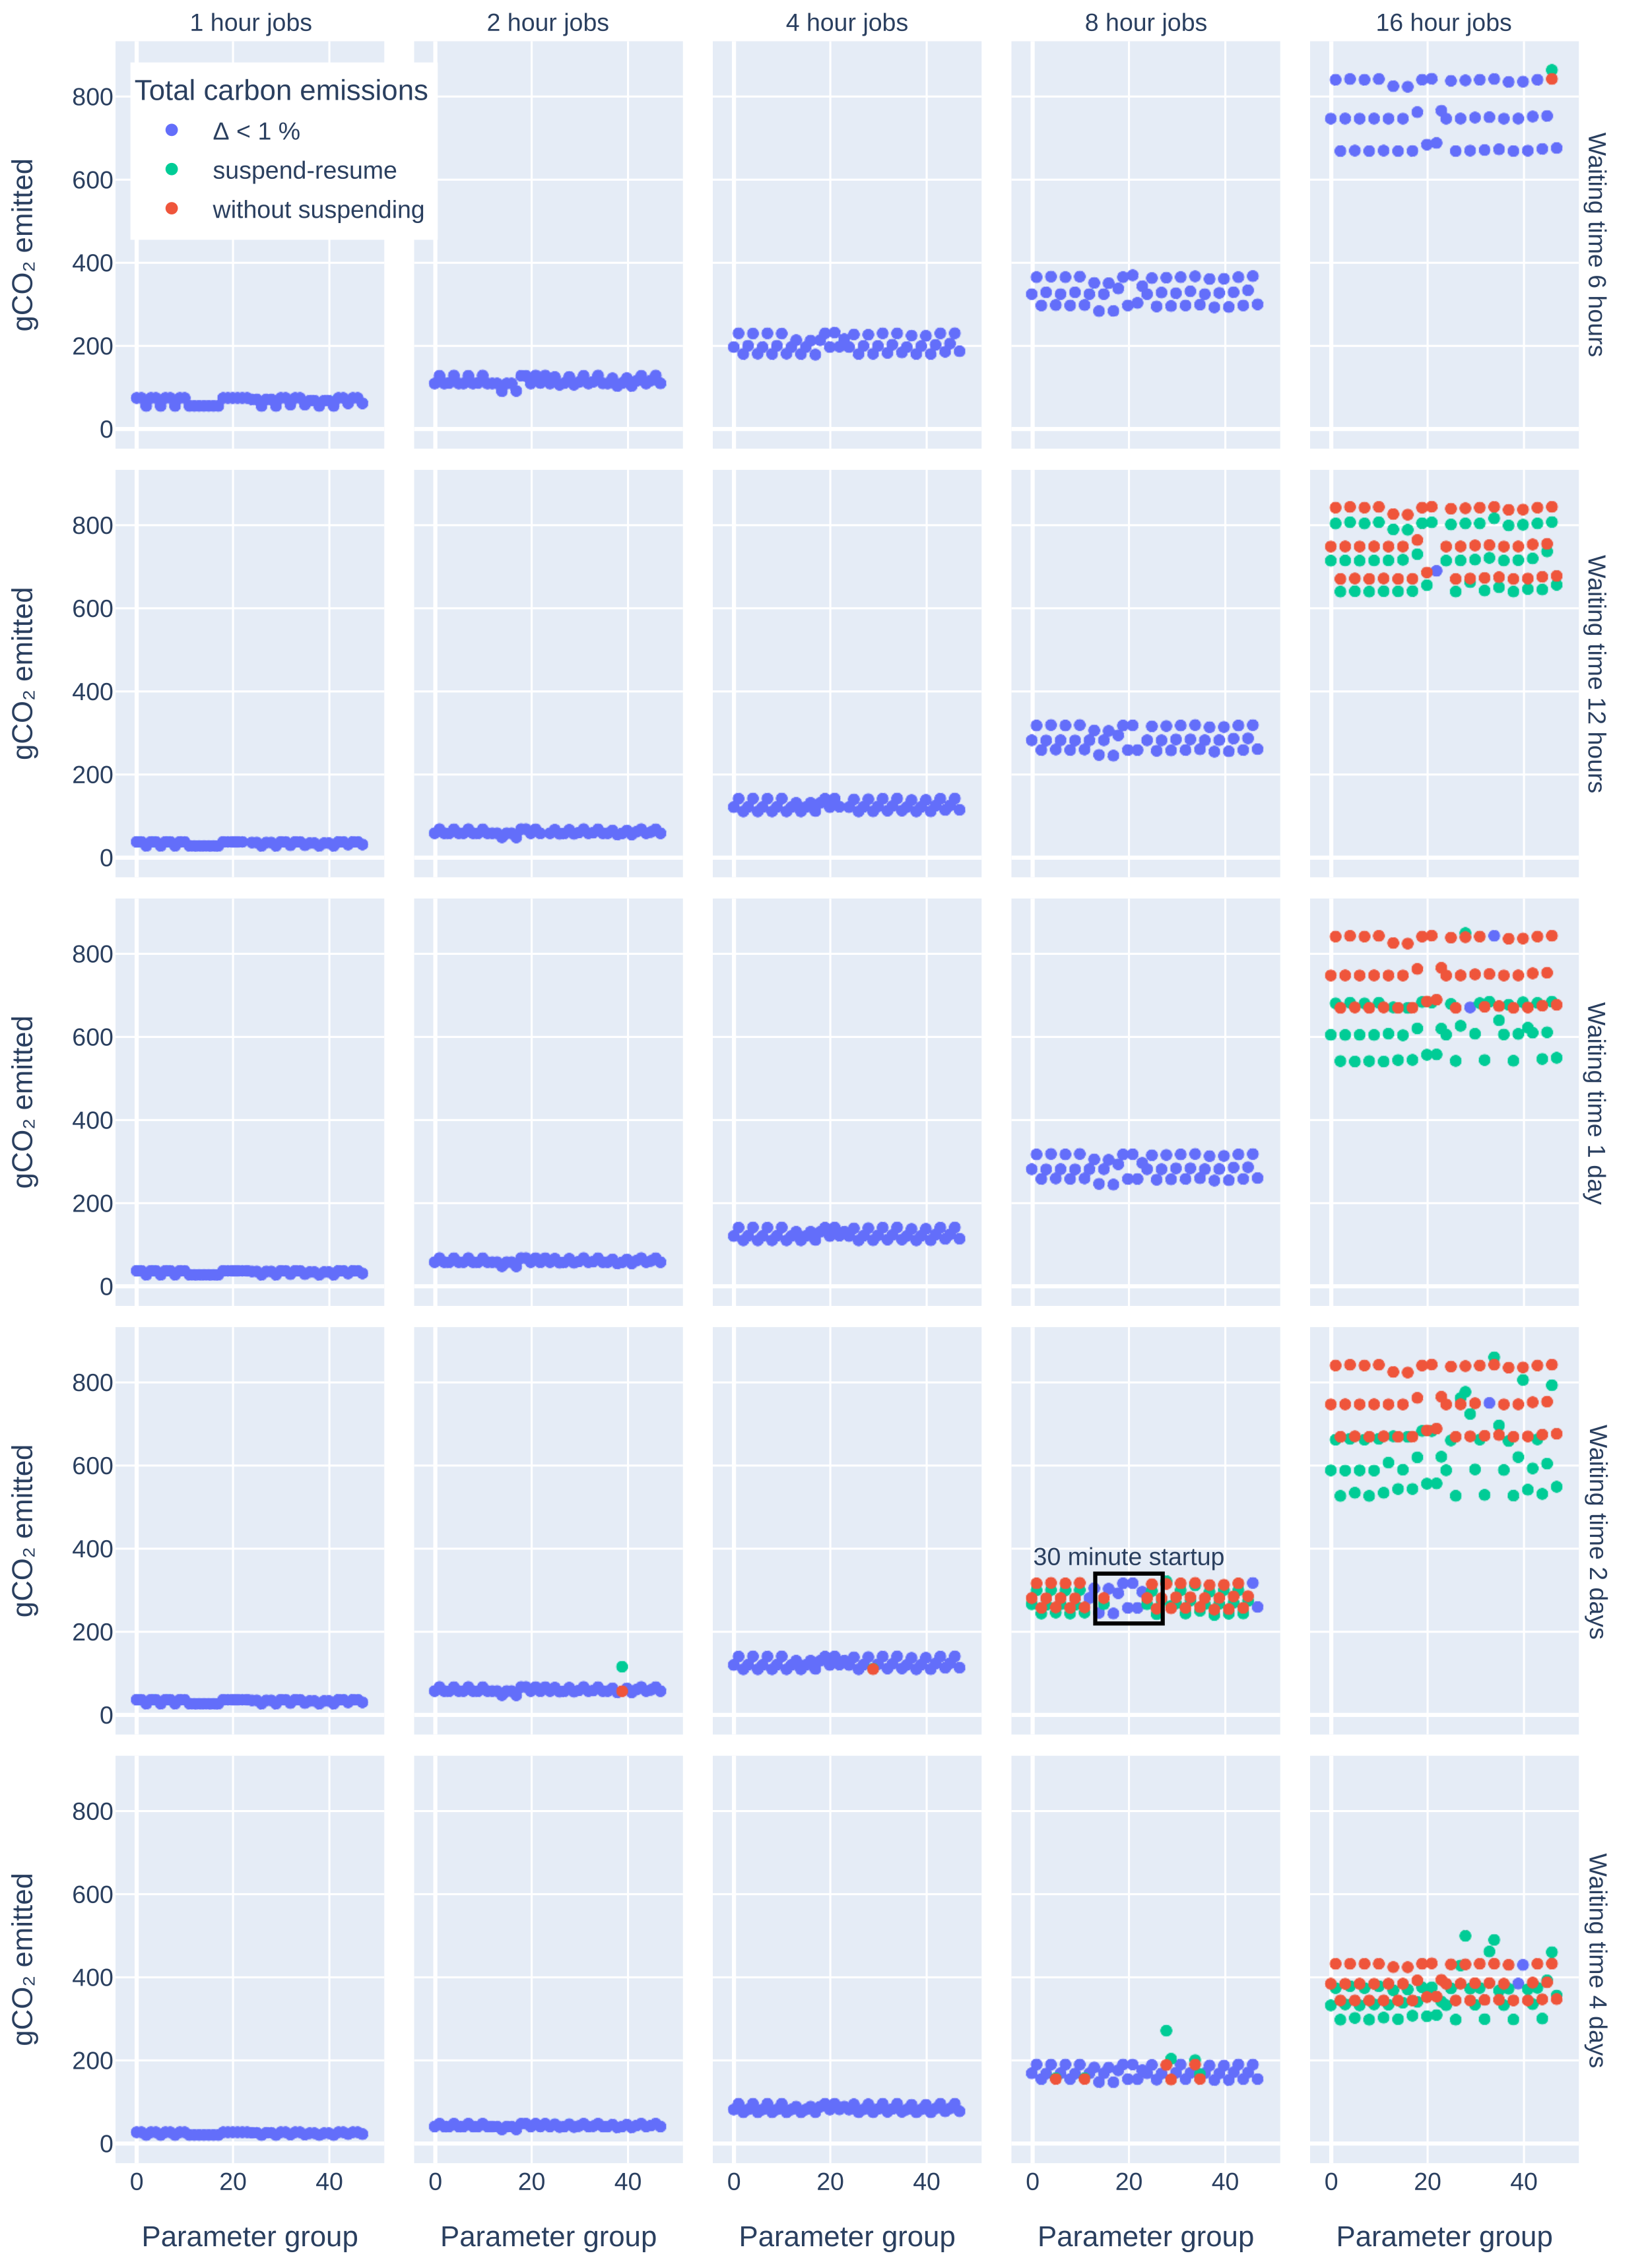
\includegraphics[width=\linewidth]{carbs/notebooks/eval_same_job_different_schedulers.pdf}
    \caption[short]{All simulated jobs and their total carbon emissions, compared between the two scheduling approaches. Blue indicates equal emissions, red and green differentiate the schedulers. The combination of startup length, startup power and phases is encoded on the horizontal axis. Savings from adopting a suspend \& resume strategy are only noticeable for very long jobs with long waiting times.}
    \label{fig:eval_different_schedulers}
\end{figure}

Since half of the 2400 jobs are LP-scheduled, about a sixth of them did not find an optimal solution in time.

\begin{figure}[H]
    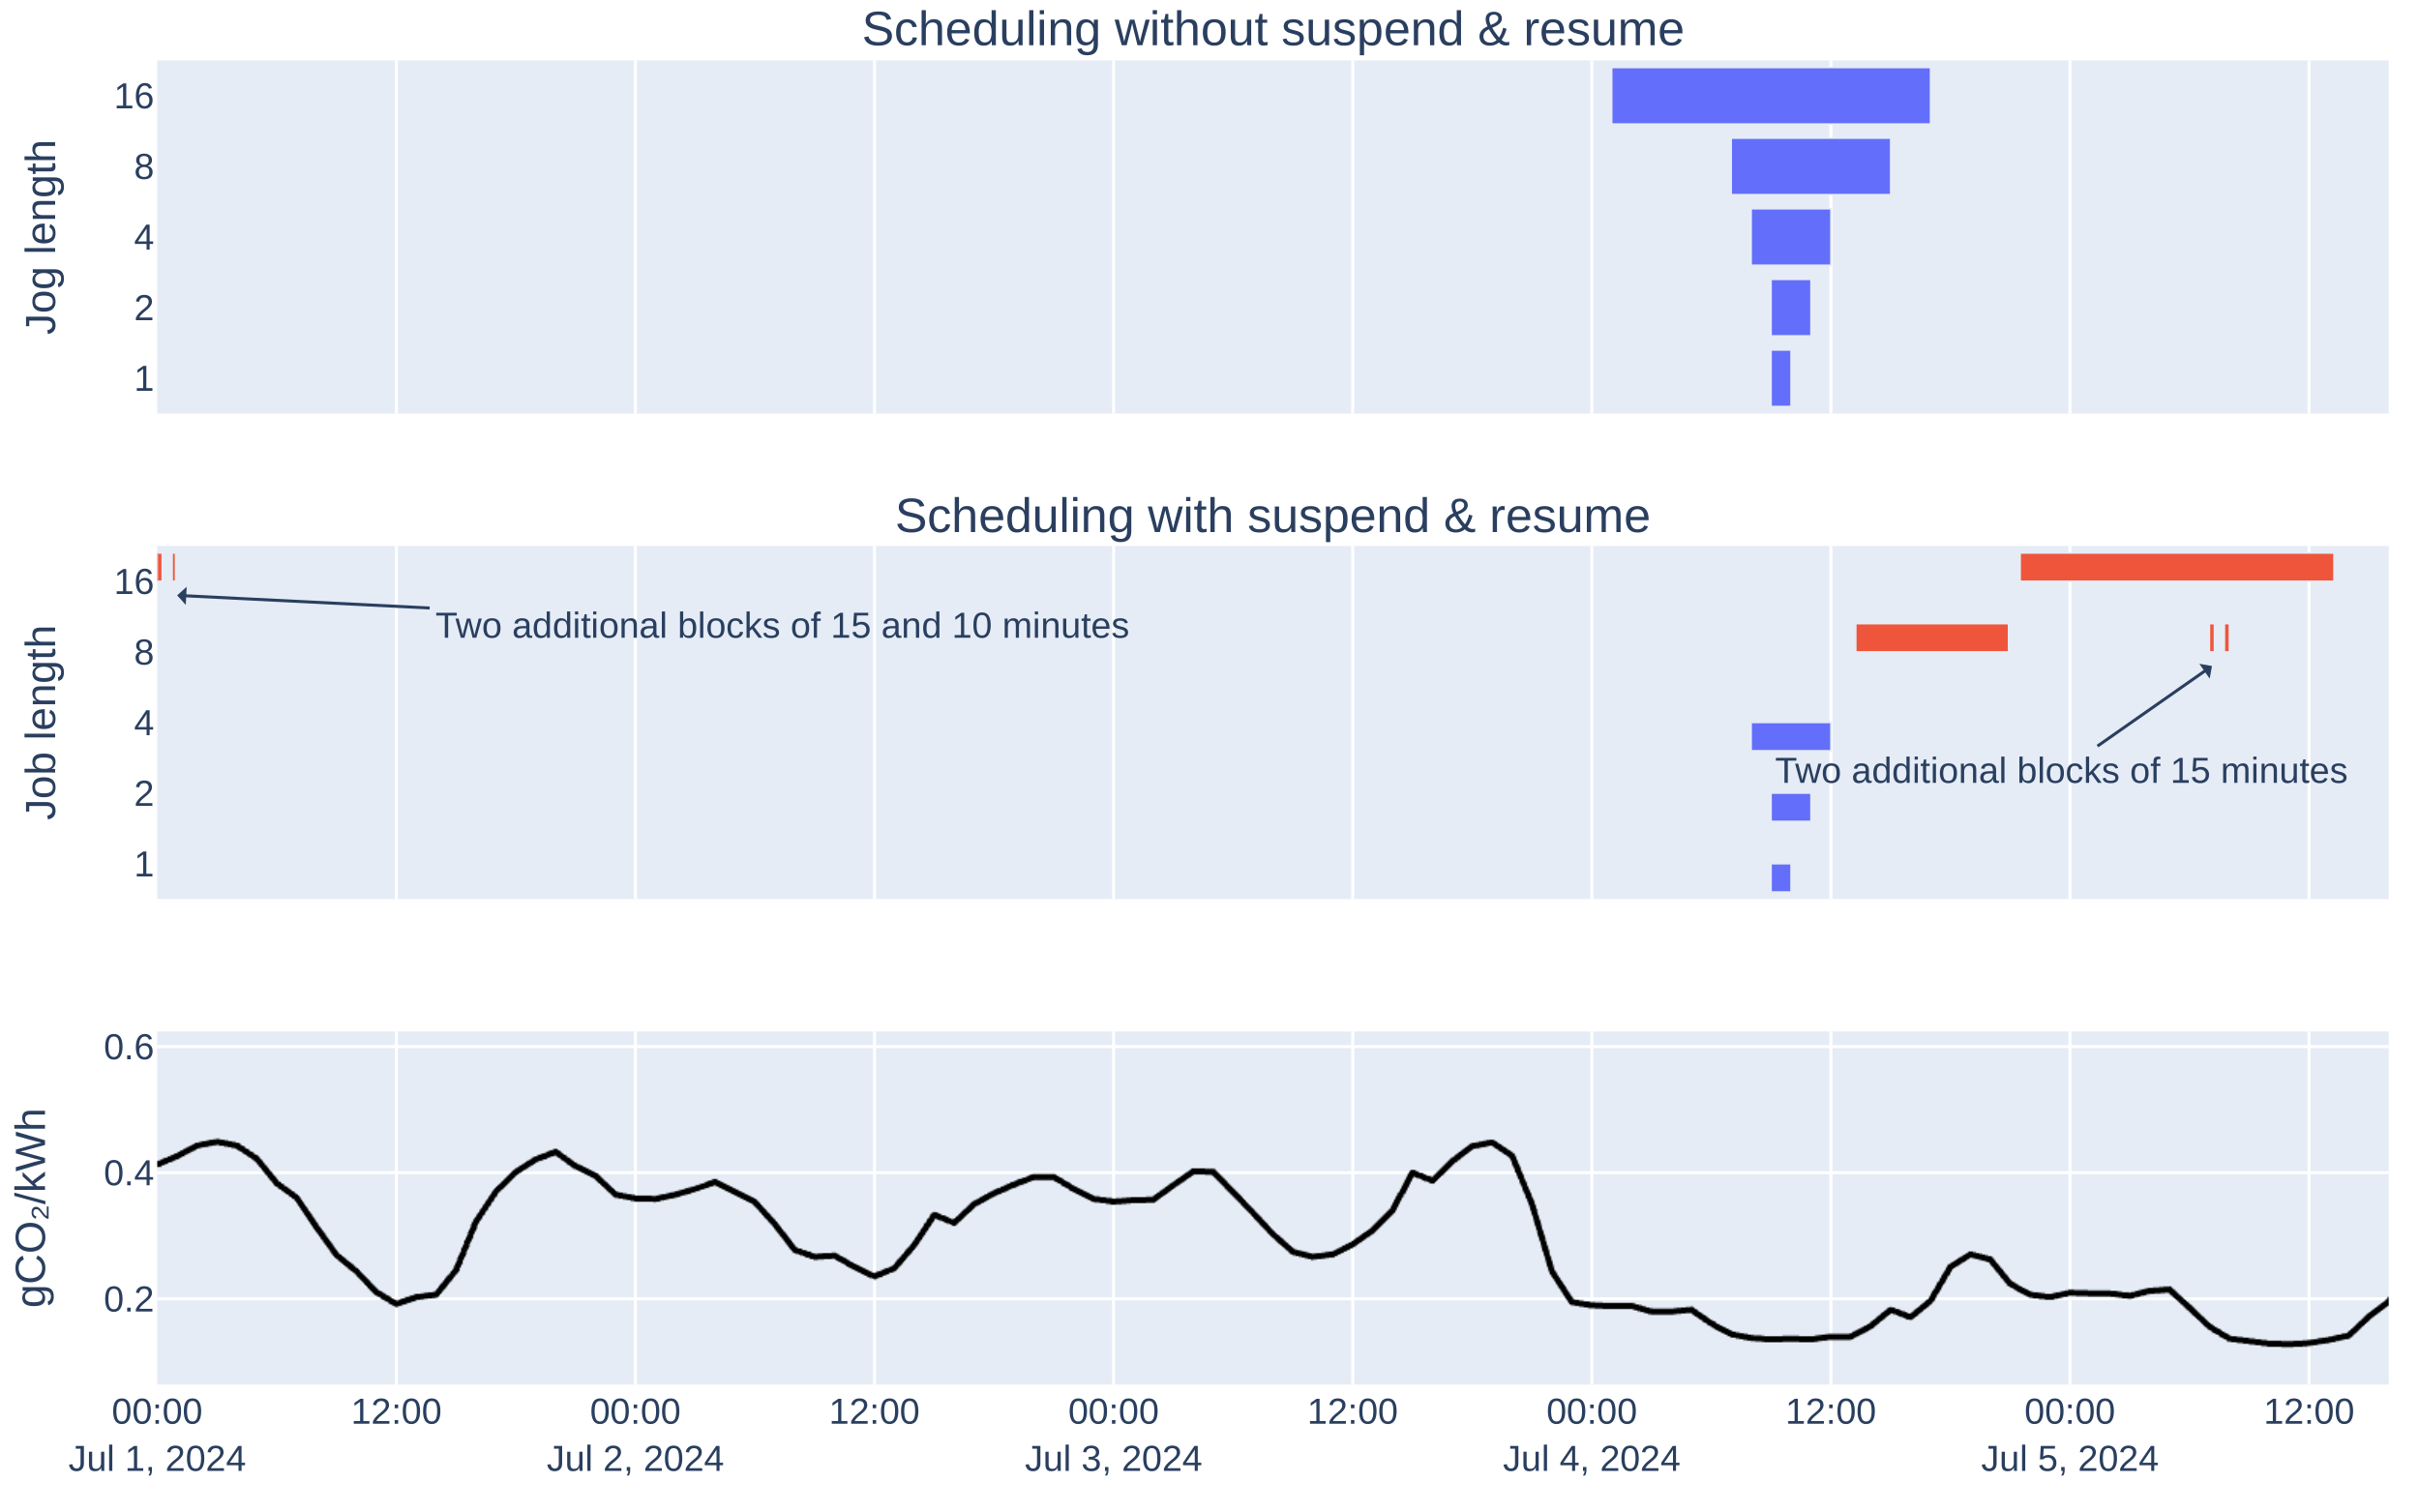
\includegraphics[width=\linewidth]{carbs/notebooks/timelimited_gantt.pdf}
    \caption[short]{Schedules of jobs sharing all parameters but length under different schedulers. All jobs have a waiting time of 4 days and a startup time of 5 minutes and an uneven phase configuration. The red bars are suboptimal schedules that are found upon being time limited.}
    \label{fig:timelimited_gantt}
\end{figure}

The cumulative distribution for the time limited solutions in Figure \ref{fig:ecdf_gap} shows a heavy skew towards bad solutions, if the time limit is not kept.

\begin{figure}[H]
    \includegraphics[width=\linewidth]{carbs/slurmlogs/gap_value_ecdf.pdf}
    \caption[short]{Cumulative distribution plot of the 209 gap values of time limited schedules. A higher gap indicates worse results. There is a heavy skew to 100\%, with half of the values being above 95\%}
    \label{fig:ecdf_gap}
\end{figure}

Despite this, the jobs with a constant power draw and startup costs were still being scheduled optimally according to the logs. 

\paragraph{Effect of Phases}

To determine whether the differences in power introduced by \modelname{} enable improvements in carbon-aware scheduling, we will use a similar approach to before. We hypothesized that in suspend \& resume scheduling, high-powered phases could be scheduled to the best slots.

\newpage
For Figure \ref{fig:different_phases_no_effect_lol}, we compare each parameter configuration between having a constant power and differing power. Taking the previous assumption of constant power as a baseline, the color of each data point represents the change in carbon in percent. As the scale of the figure suggests, most jobs did not exert meaningful changes in emissions. 

\begin{figure}[H]
    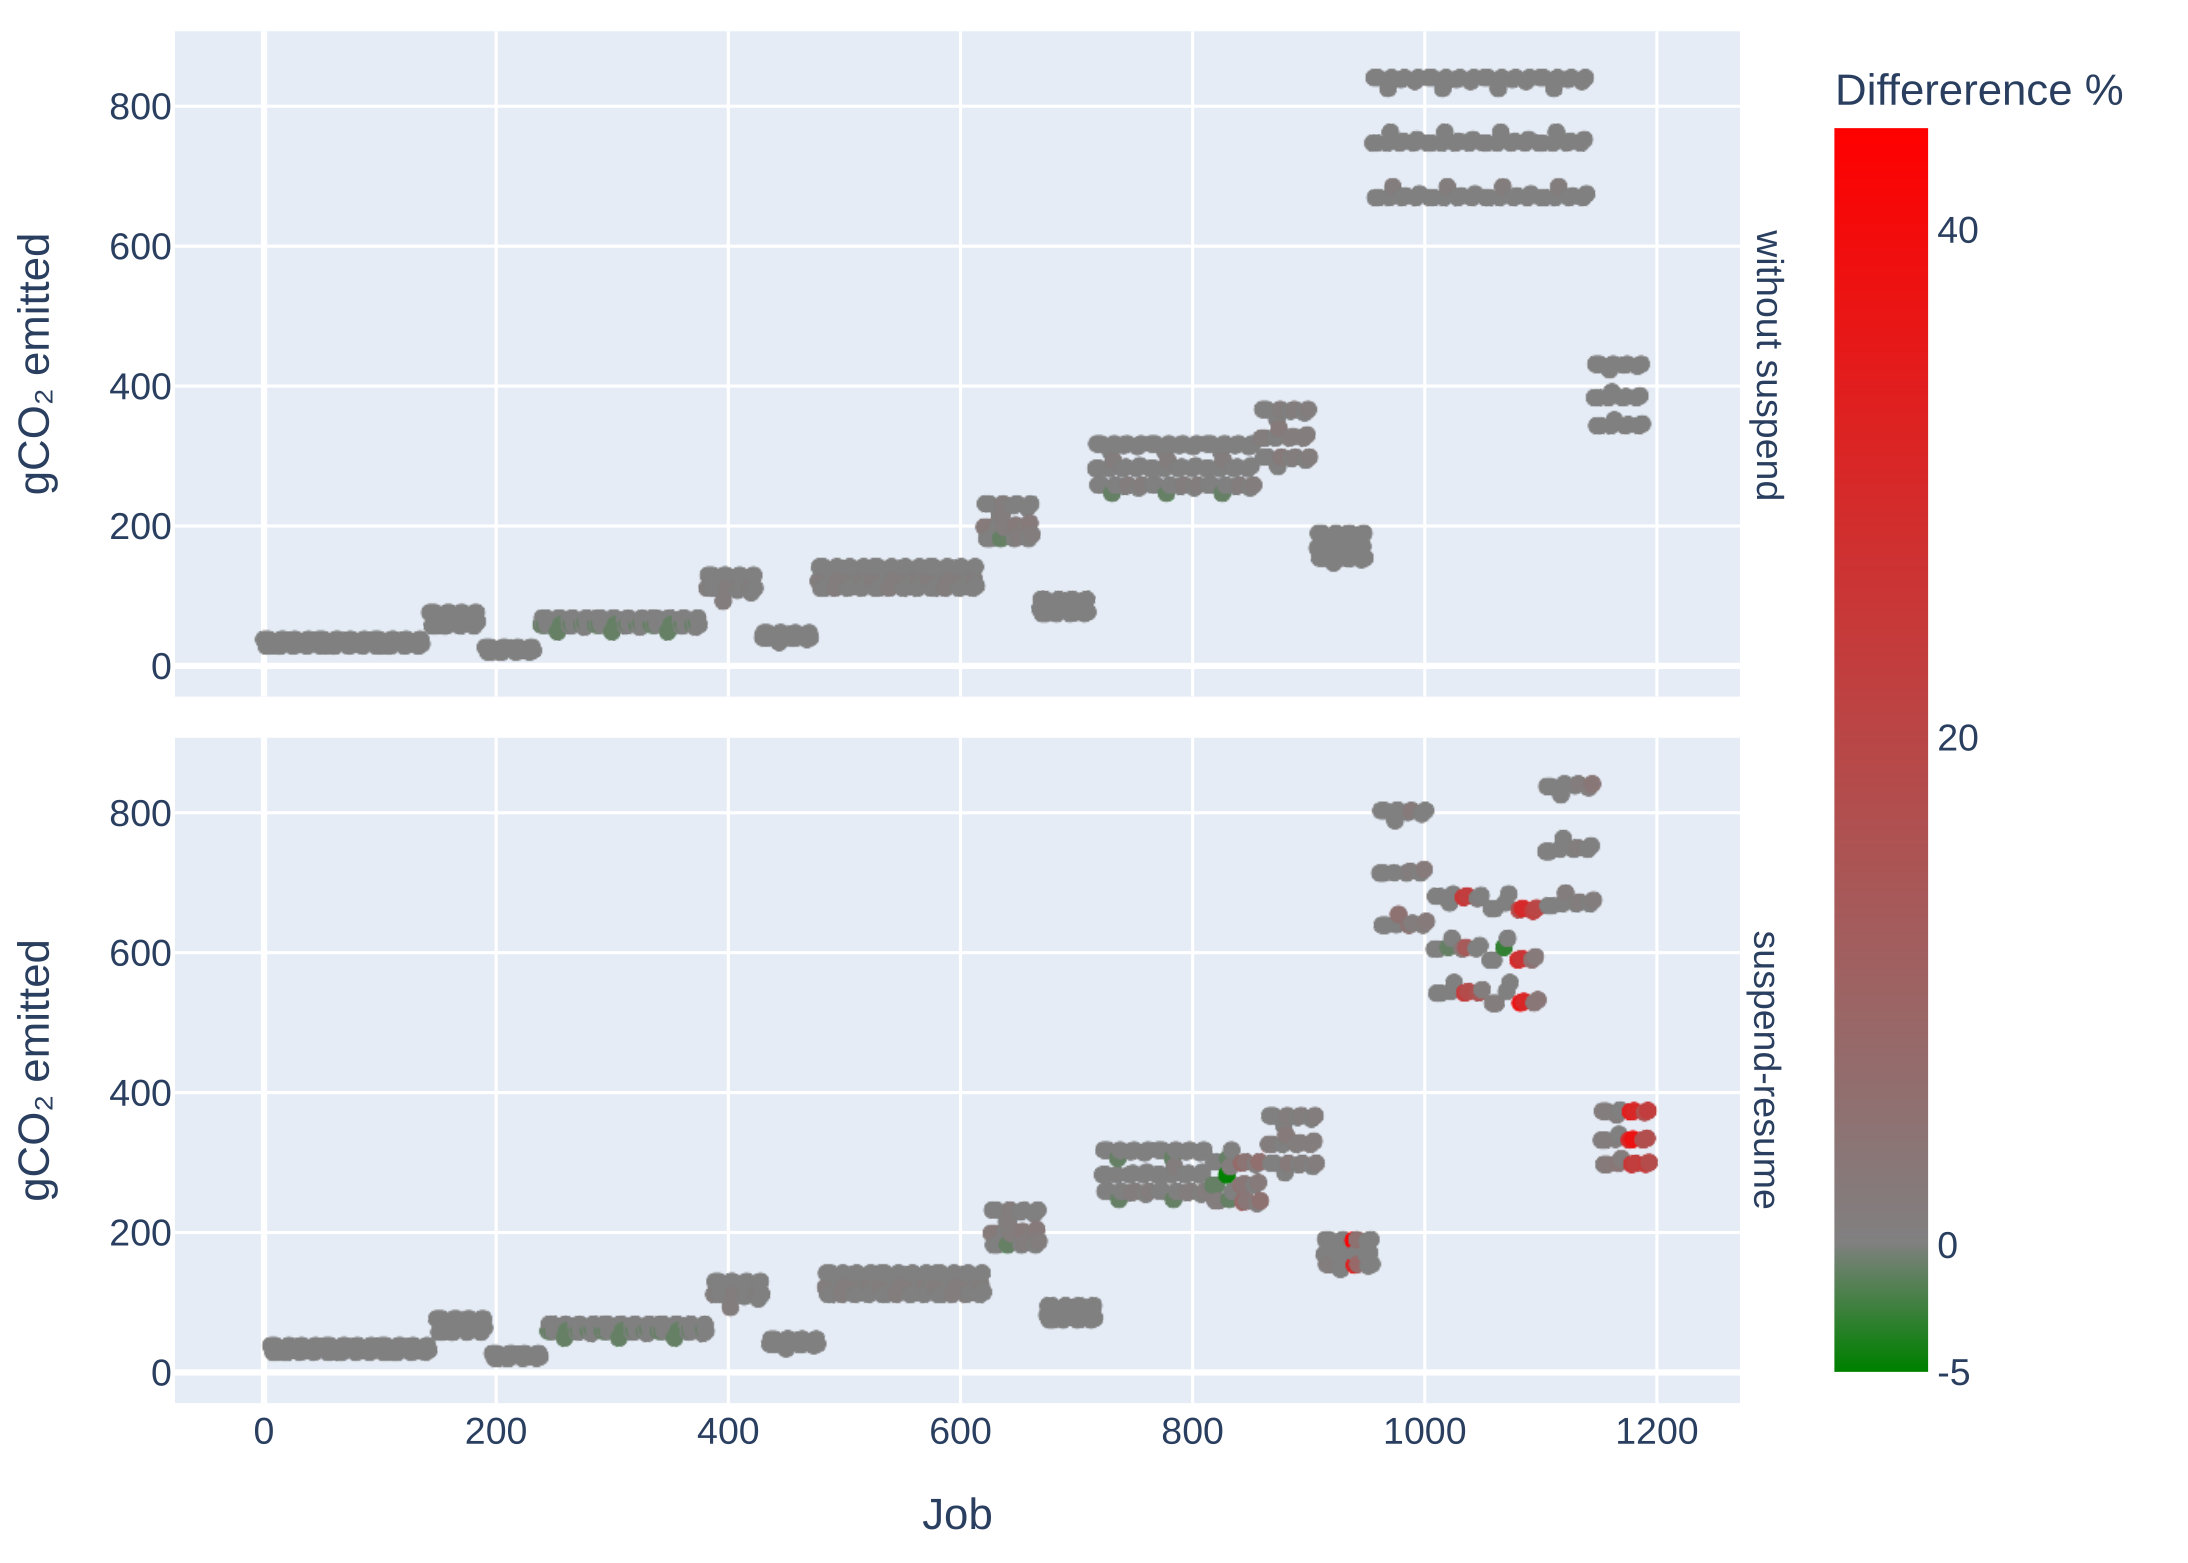
\includegraphics[width=\linewidth]{carbs/notebooks/eval_same_job_different_phases.pdf}
    \caption[short]{Difference in carbon emissions from having heterogeneous phases compared to the baseline of a constant average. For the majority of jobs, this had an effect of ±1\%. Red signifies jobs, where this increased carbon emissions. For suspend \& resume scheduling, some jobs had highly increased emissions. These are likely the result of to time-outs due to increased complexity.}

    \label{fig:different_phases_no_effect_lol}
\end{figure}

Opposite to our intention, some jobs had highly increased carbon emissions from gaining a more detailed power profile.
One explanation we suggest is the same as for the increased emissions in the scheduler comparison before: scheduling long jobs with long deadlines lead to timeout due to the increased complexity from having different phases. 
For each such job, the same configuration with a constant assumption would be able to find an optimal schedule, while a non-constant assumption would not.

Even for jobs that found an optimal schedule, the savings are minimal, if any. 
This is likely due to the design of the evaluation: with a resolution of an hour for the carbon emissions and the phases sharing that resolution, the averaged power is likely too close on this scale. Another reason could be that the chosen carbon trace exhibits a very \emph{wavy} pattern. Unlike the Australian trace used in Section \ref{sec:checkpoint_resume_lp}, the German trace used for this evaluation had fewer sudden shifts in carbon intensity, likely making scheduling according to phases less worthwhile.

\paragraph{Effect of Waiting Times}

Figure \ref{fig:different_deadlines_normalized} shows the carbon emissions for each job across different waiting times.
We decided to remove the heterogeneous jobs from these plots, as the chosen parameters had little effect on emissions, instead only causing timeouts. 
Across the remaining parameters, the relative carbon savings are very close, showing up as a single dot.
In two instances, there were changes, however.
For longer jobs with a waiting time of 2 days, having a startup time of half an hour decreased relative savings. 

\begin{figure}[H]
    \includegraphics[width=\linewidth]{carbs/notebooks/normalized_deadlines.pdf}
    \caption[short]{
        Normalized carbon emissions with the baseline being a wait time of 6 hours for each constant-power job. 
        There are small difference for jobs with a startup length of 30 minutes but for the most part, there is no difference across the remaining parameters.
    }

    \label{fig:different_deadlines_normalized}
\end{figure}

Jobs shorter than 16 hours had stagnating savings beyond a waiting time of 12 hours. 
It is likely, that this is a circumstance of the chosen carbon trace.
The best period is around noon on July 1 (see the bottom graph of Figure \ref{fig:timelimited_gantt}), which also fits shorter job lengths. 
With a 4 days waiting time, shorter jobs could then again be scheduled on the new lowest carbon emissions period.

\paragraph{Summary}

As for our given research questions, answering them under the current evaluation cannot be done definitively. We found that, within a summer week in Germany, longer jobs have a higher potential for carbon savings using a suspend \& resume strategy, even if resuming a job carries overhead. Increasing the deadline for a given job also displays a trend of increasing carbon reduction. 
Very long jobs, in this case 16 hours, exhibit higher saving potential from waiting times.
The effect of workload heterogeneity is unclear, as the chosen phase scenarios, of (short) alternating phases, likely do not have significant saving potential inherently.

On the other side, we have gained insights into the limitations of suspend \& resume scheduling in \programname{}. Specifically, scheduling certain workloads - those with many alternating phases, long runtimes, and deadlines - has long runtimes.
In Section \ref{sec:discussion}, we will give ideas for a better-suited evaluation.
